\documentclass[main.tex]{subfiles}
\pagestyle{main}

\begin{document}

%%%% Warning : les coupures se basent sur le fait que les images font 888*888

%%%%% Evo aire NBER+EXON
\begin{figure}[ht]
\subfloat[Patient A: profile that has a good reponse to the treatment.]{\label{fig_henbert}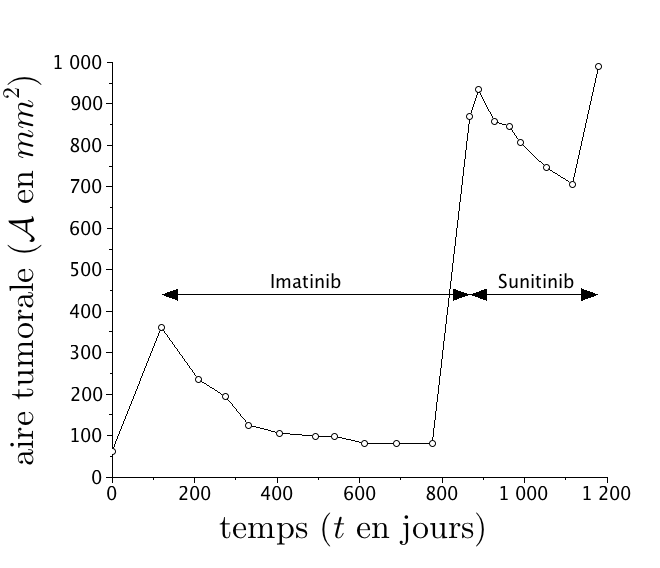
\includegraphics[width=0.5\textwidth]{henbert.png}}
\subfloat[Patient E: typical profile of resistance to imatinib
associated to a particular genetic KIT mutation (reported in EXON11).]{\label{fig_brio_ckit}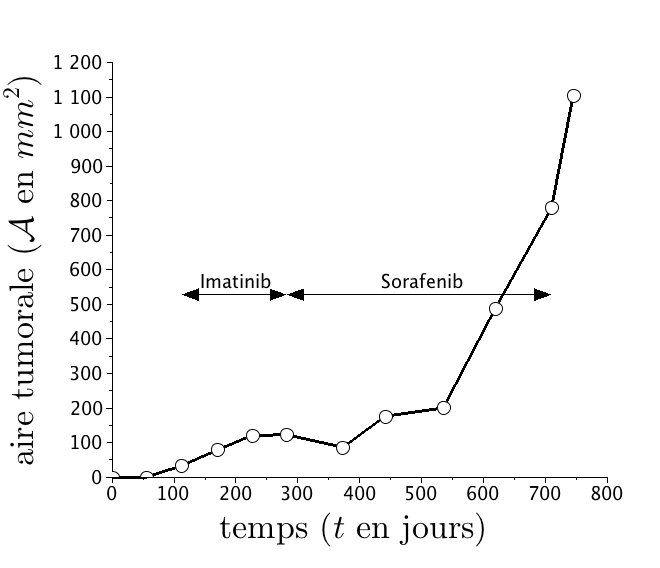
\includegraphics[width=0.5\textwidth]{brio.png}}
\caption{Evolution of GIST metastases of  two differents patients. \\ Figure~\ref{fig_henbert} is representative of the most common evolution of GIST metastases, while Figure~\ref{fig_brio_ckit} presents the typical evolution of tumors with a genetic mutation.}
\end{figure}

%%%%%% scan NBER
\begin{figure}
\subfloat[Sept 16, 2008 -- Day 119]{\label{fig_hen_spatial_1}
\reshapeimg{1.0}{0px}{0px}%
\tikzzoom{full_scan/scan_henbert/2008_09_16(2).jpg}{3}{1.5}{1.2}%
}
\subfloat[June 30, 2009 -- Day 406]{\label{fig_hen_spatial_2}
\reshapeimg{1.1}{0px}{-9px}%
\tikzzoom{full_scan/scan_henbert/2009_06_30(2).jpg}{3}{1.6}{1.2}%
}
\subfloat[July 5, 2010  -- Day 776]{\label{fig_hen_spatial_3}
\reshapeimg{1.1}{0px}{28px}%
\tikzzoom{full_scan/scan_henbert/2010_07_05(3).jpg}{3}{1.5}{1.0}%
}
\\
\subfloat[Oct 25, 2010 -- Day 888]{\label{fig_hen_spatial_4}
\reshapeimg{1.28}{45px}{50px}%
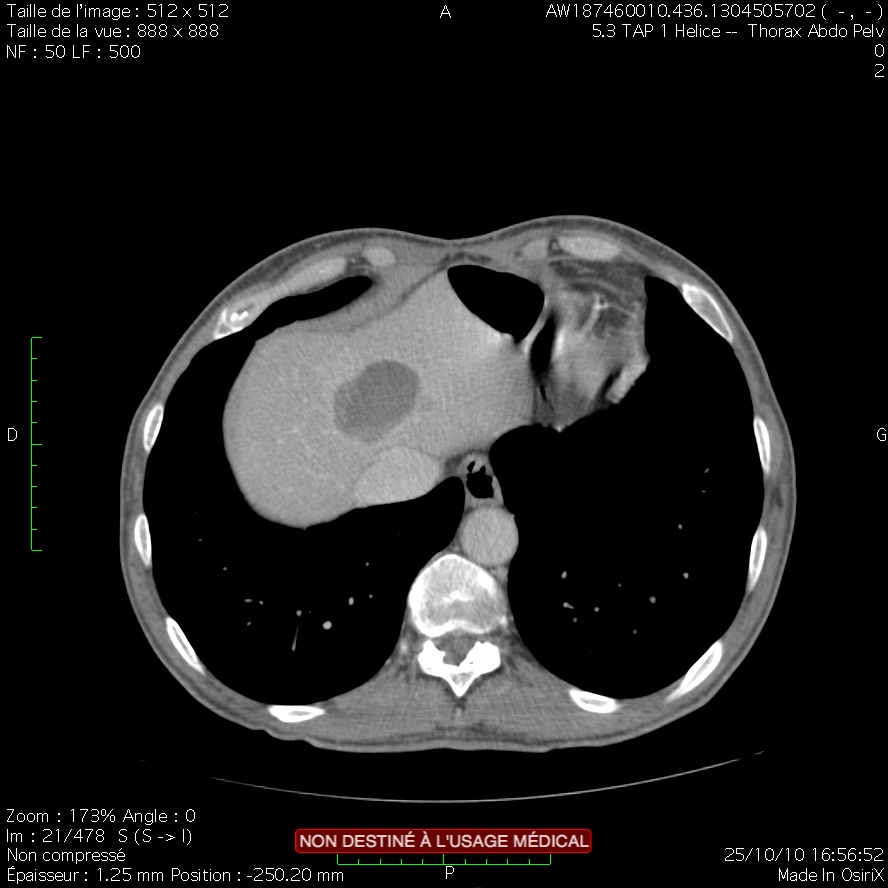
\includegraphics[trim = {\margg} {\margb} {\margd} {\margh}, clip, width=0.32\textwidth]{full_scan/scan_henbert/2010_10_25.jpg}%
}
\subfloat[Jan 7, 2011 -- Day 962]{\label{fig_hen_spatial_5}
\reshapeimg{1.11}{20px}{-66px}%
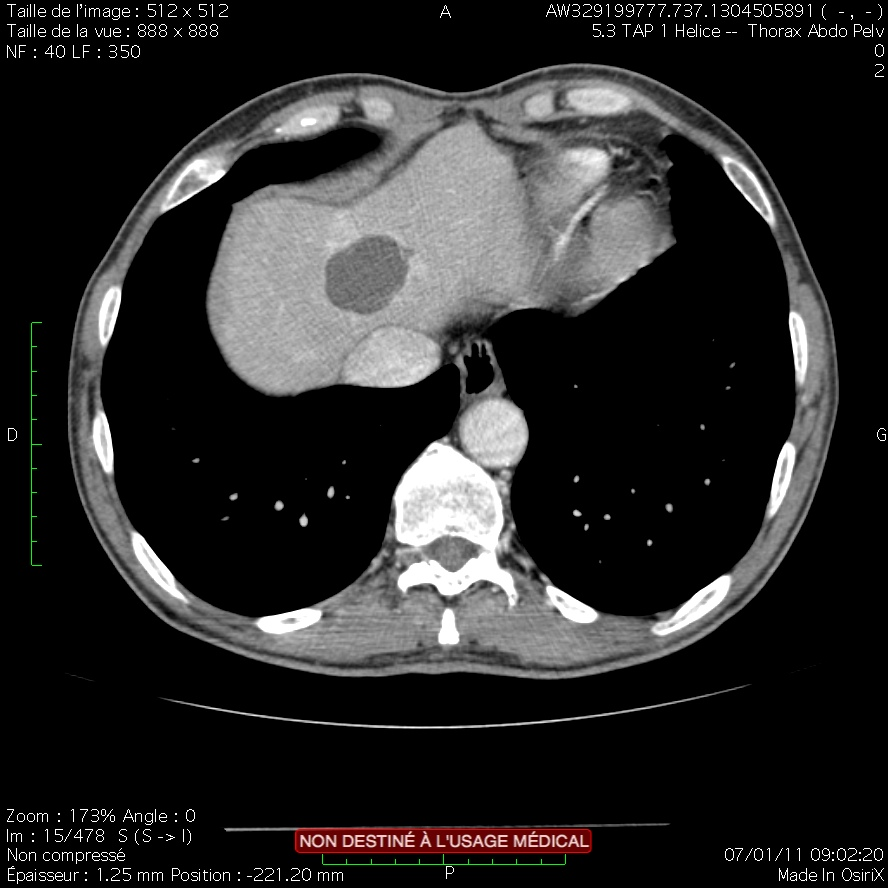
\includegraphics[trim = {\margg} {\margb} {\margd} {\margh}, clip, width=0.32\textwidth]{full_scan/scan_henbert/2011_01_07(2).jpg}%
}
\subfloat[June 10, 2011 -- Day 1116]{\label{fig_hen_spatial_6}
\reshapeimg{1.28}{50px}{-8px}%
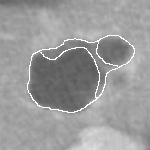
\includegraphics[trim = {\margg} {\margb} {\margd} {\margh}, clip, width=0.32\textwidth]{full_scan/scan_henbert/2011_06_10.jpg}%
}
\caption{\label{fig_hen_spatial}Spatial evolution of the liver 
    metastasis of patient A on a series of CT-scan s.}
\end{figure}

%%%%%% Evo Masse NBER
\begin{figure}
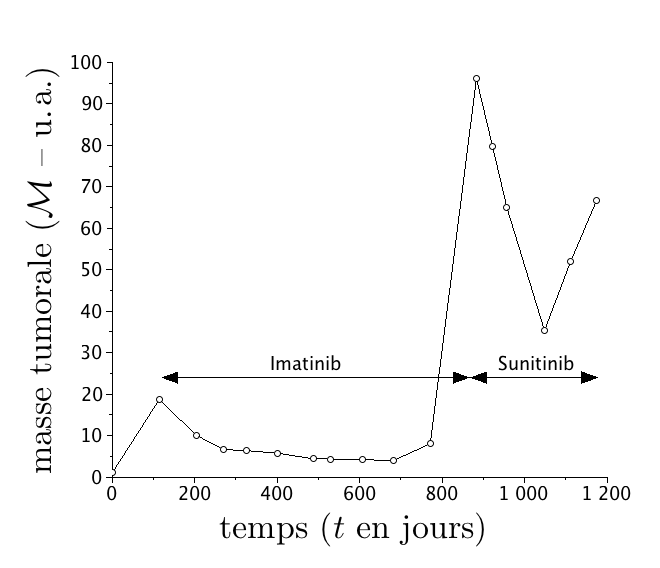
\includegraphics[width=0.45\textwidth]{masses_NBER.png}
\caption{Patient A: tumor mass evolution (normalization of
    integral of grey levels) with respect to time (in days).
%(number of cancer cells as a fonction of time in days) %of the case presented in Figure~\ref{fig_henbert}.
\label{fig_mass_henbert}}
\end{figure}

%%%%%%% Taux de croissance
%\begin{figure}
%\centering
%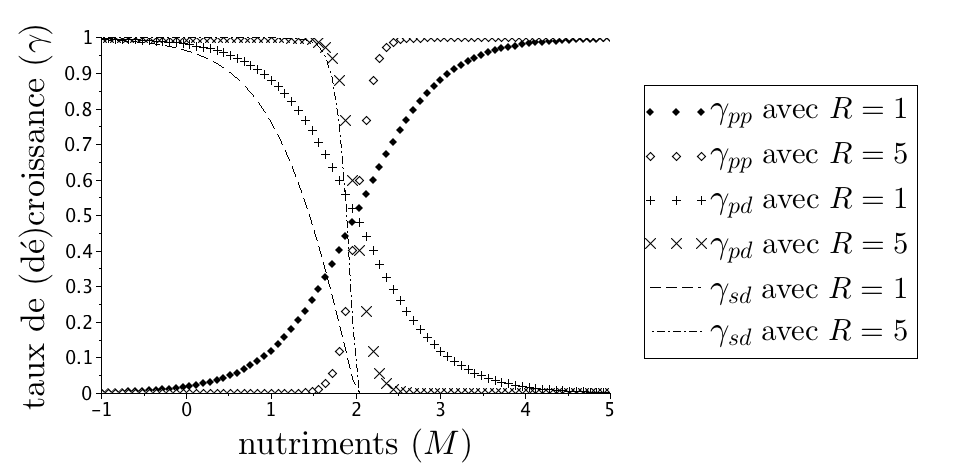
\includegraphics[width=0.75\textwidth]{gamma_v2.png}
%\caption{\textbf{Growth rate and decreasing rate of the cells.}\\
%Here $\gamma_0=\gamma_1=C_S=1$ and $\Ms = 2$. -- Units are arbitrary. \label{fig:gamma}}
%\end{figure}




%%%%%%%%%% Scan Chen
\begin{figure}[p]
\subfloat[May 23, 2007 -- Day 0]{\label{fig_chen_spatial_1}
\reshapeimg{1.05}{0px}{0px}%
\tikzzoom{full_scan/scan_chen/2007_mai_23.jpg}{4}{0}{2.1}%
%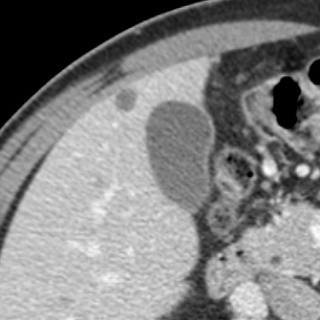
\includegraphics[trim = {\margg} {\margb} {\margd} {\margh}, clip, width=0.32\textwidth]{full_scan/scan_chen/2007_mai_23.jpg}%
}
\subfloat[July 25, 2008 -- Day 429]{\label{fig_chen_spatial_2}
\reshapeimg{1.0}{0px}{-20px}%
\tikzzoom{full_scan/scan_chen/2008_juil_25.jpg}{4}{-0.15}{1.95}%
%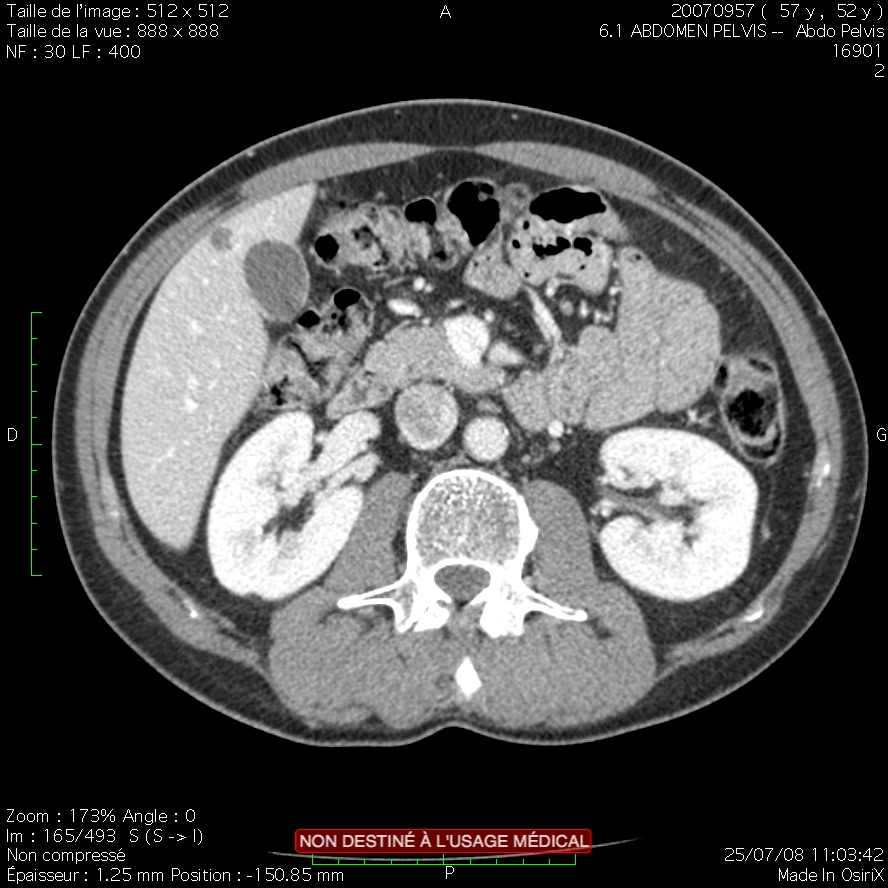
\includegraphics[trim = {\margg} {\margb} {\margd} {\margh}, clip, width=0.32\textwidth]{full_scan/scan_chen/2008_juil_25.jpg}%
}
\subfloat[Sept 14, 2009 -- Day 845]{\label{fig_chen_spatial_3}
\reshapeimg{1.25}{80px}{-40px}%
%\tikzzoom{full_scan/scan_chen/2009_sept_14.jpg}{3}{1.7}{1.15}%
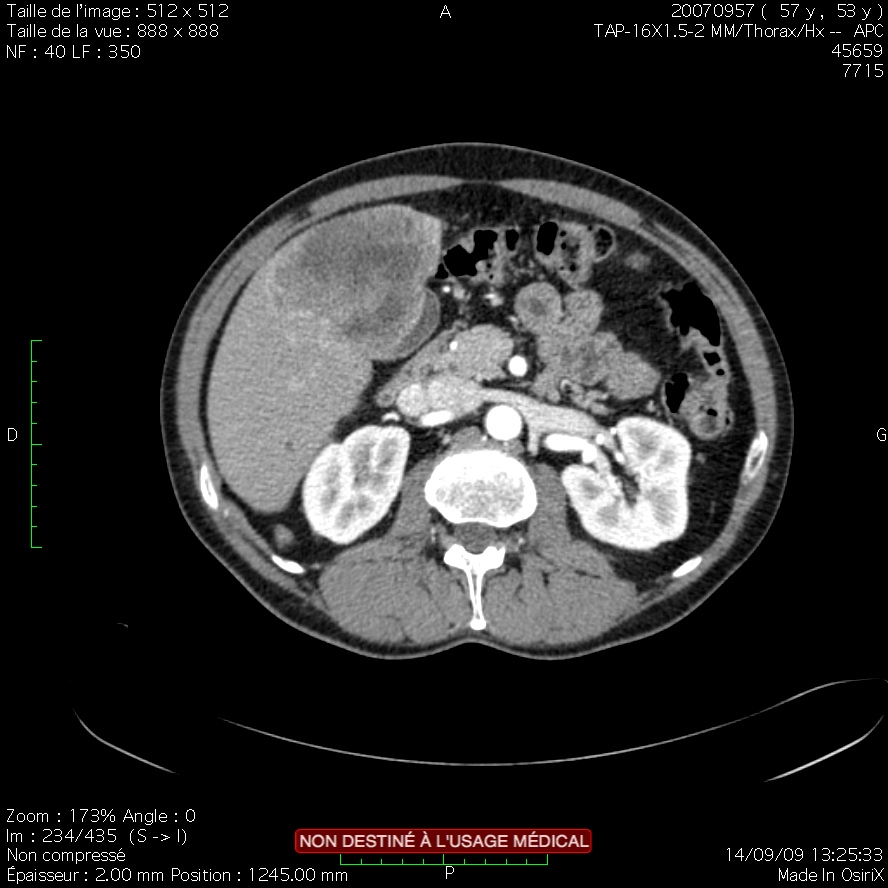
\includegraphics[trim = {\margg} {\margb} {\margd} {\margh}, clip, width=0.32\textwidth]{full_scan/scan_chen/2009_sept_14.jpg}%
}
\\
\subfloat[April 06, 2010 -- Day 1049]{\label{fig_chen_spatial_4}
\reshapeimg{1.15}{45px}{0px}%
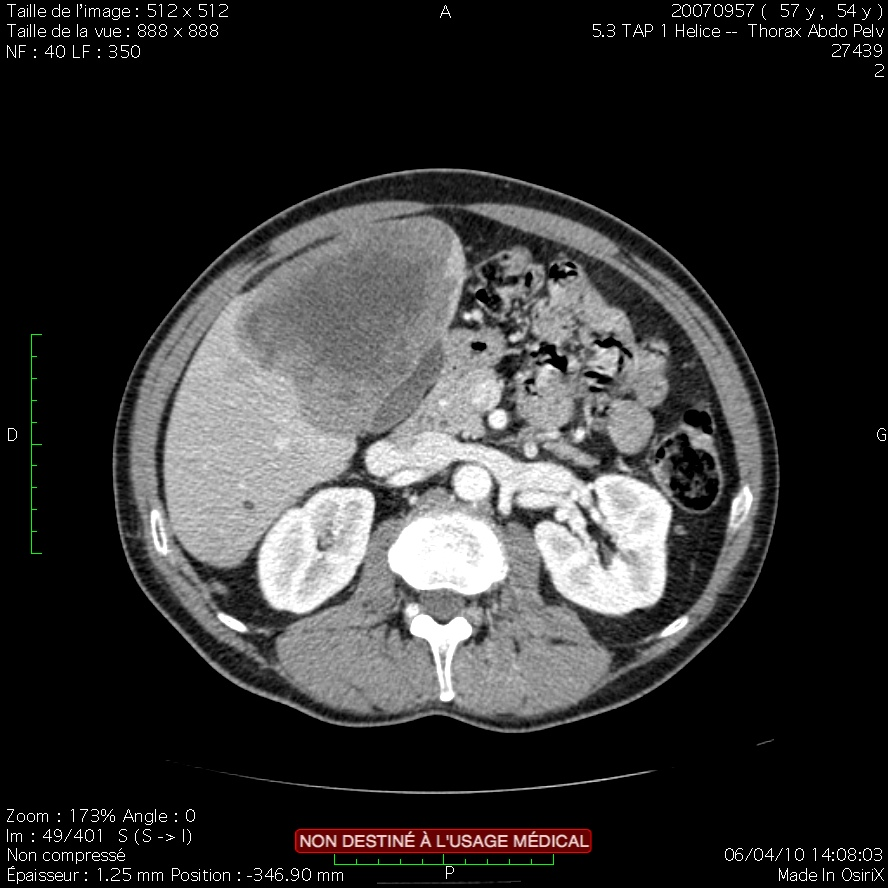
\includegraphics[trim = {\margg} {\margb} {\margd} {\margh}, clip, width=0.32\textwidth]{full_scan/scan_chen/2010_avril_06.jpg}%
}
\subfloat[Sept 28, 2010 -- Day 1224]{\label{fig_chen_spatial_5}
\reshapeimg{1.05}{35px}{-40px}%
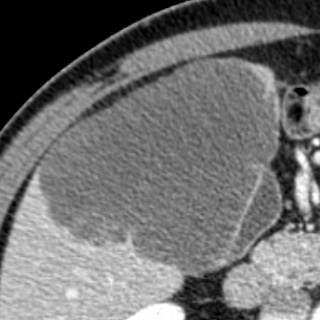
\includegraphics[trim = {\margg} {\margb} {\margd} {\margh}, clip, width=0.32\textwidth]{full_scan/scan_chen/2010_sept_28.jpg}%
}
\subfloat[May 20, 2011 -- Day 1458]{\label{fig_chen_spatial_6}
\reshapeimg{1.05}{50px}{-8px}%
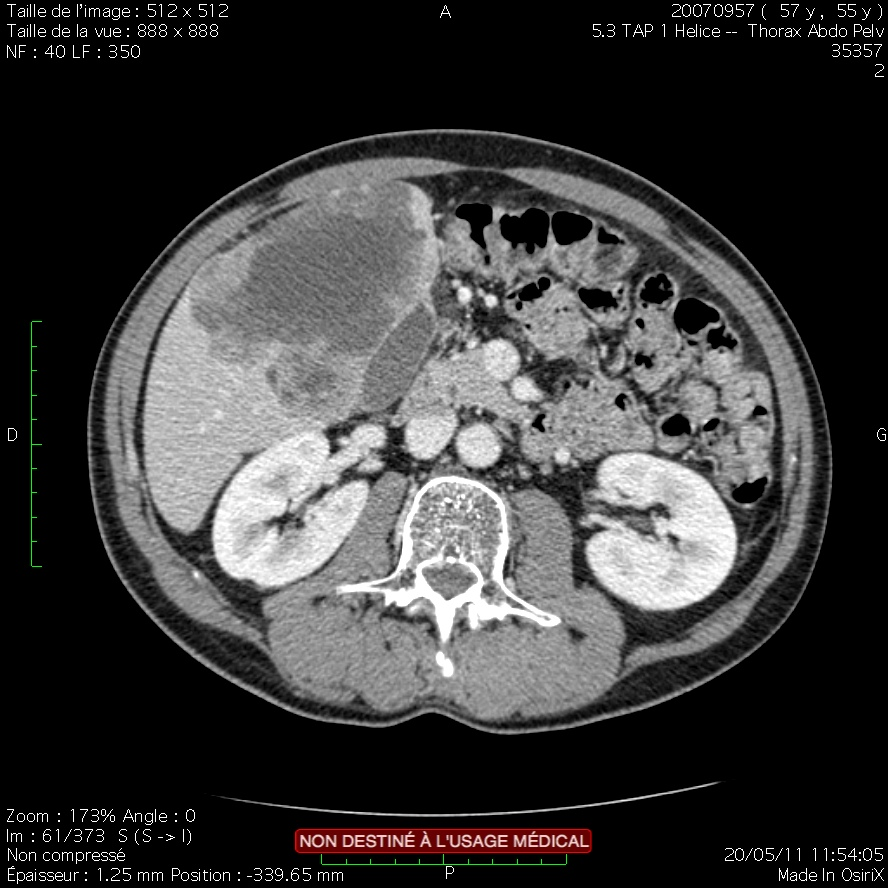
\includegraphics[trim = {\margg} {\margb} {\margd} {\margh}, clip, width=0.32\textwidth]{full_scan/scan_chen/2011_mai_20.jpg}%
}
\caption{\label{fig_chen_spatial} Spatial evolution of the patient B metastasis on a series of CT-scans.}
\end{figure}

%%%%%%%%% Simu Chen spatial a priori
\begin{figure}[!ht]
%%%% simu  trefle_track/point3.0/track_10x10_7
%\vspace{-56mm}
\subfloat[Day 0]{\label{fig_chen_simu_spatial_1}
\includegraphics[width=0.33\textwidth]{simu/trefle_track/point3_0/track_10x10_7/vue_scan/vue_scan1.png}}
\subfloat[Day 543]{\label{fig_chen_simu_spatial_2}
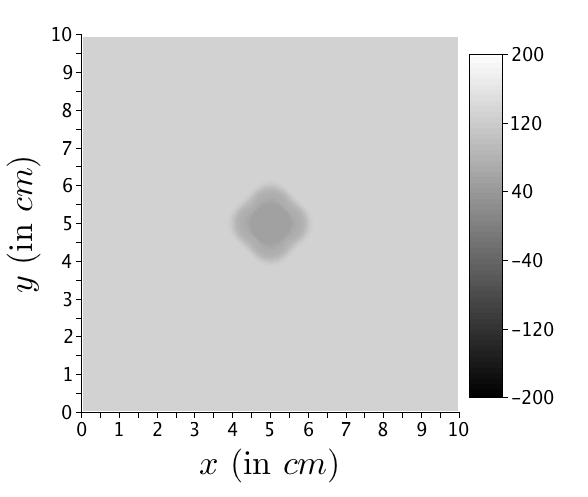
\includegraphics[width=0.33\textwidth]{simu/trefle_track/point3_0/track_10x10_7/vue_scan/vue_scan34.png}}
\subfloat[Day 724]{\label{fig_chen_simu_spatial_3}
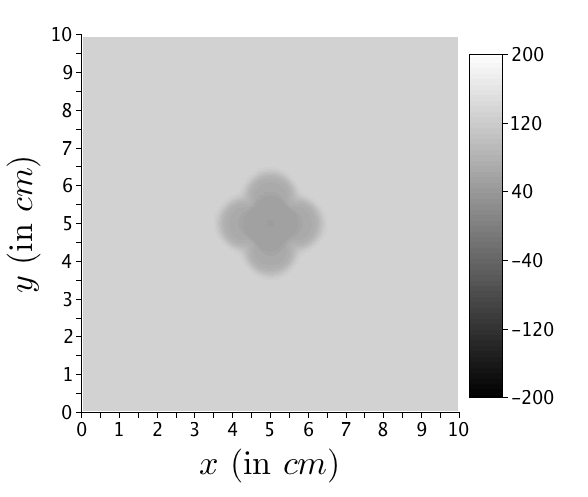
\includegraphics[width=0.33\textwidth]{simu/trefle_track/point3_0/track_10x10_7/vue_scan/vue_scan45.png}}
\vspace{-4mm}\\
\subfloat[Day 1053]{\label{fig_chen_simu_spatial_4}
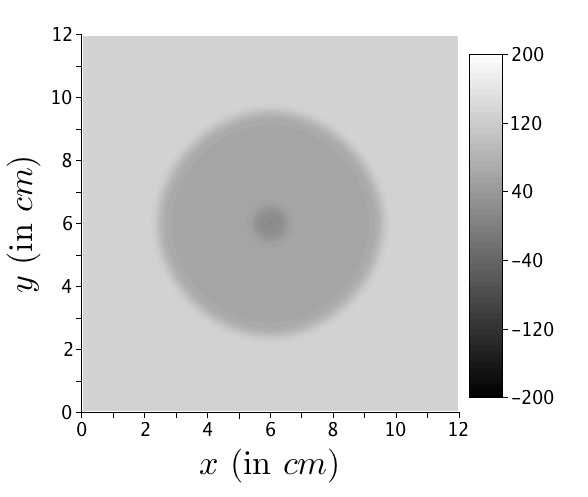
\includegraphics[width=0.33\textwidth]{simu/trefle_track/point3_0/track_10x10_7/vue_scan/vue_scan65.png}}
\subfloat[Day 1399]{\label{fig_chen_simu_spatial_5}
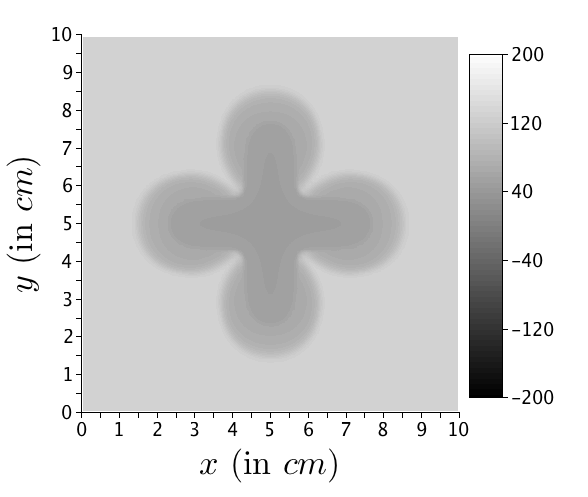
\includegraphics[width=0.33\textwidth]{simu/trefle_track/point3_0/track_10x10_7/vue_scan/vue_scan86.png}}
\subfloat[Day 1600]{\label{fig_chen_simu_spatial_6}
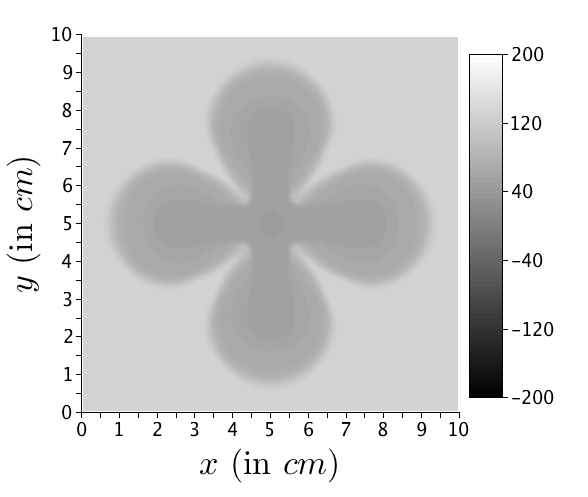
\includegraphics[width=0.33\textwidth]{simu/trefle_track/point3_0/track_10x10_7/vue_scan/vue_scan99.png}}
%\vspace{5mm}
\caption{Numerical simulations with standard WENO5 stencil  for patient B: spatial evolution of the lesion with numerical reconstitution of CT-scan s.\\
The unit of grey scale is arbitrary. \label{fig:simu_chen_cross0_scan}}
\end{figure}

\clearpage



%%%%%%%%%%% Correction twin weno
\begin{figure}[!htb]
%%\vspace{-6mm}
\subfloat[Spatial aspect of the tumor on day 1366 with numerical reconstitution of CT-scan s. The unit of grey scale is arbitrary.]{
\label{fig:correction_cross_spatial}
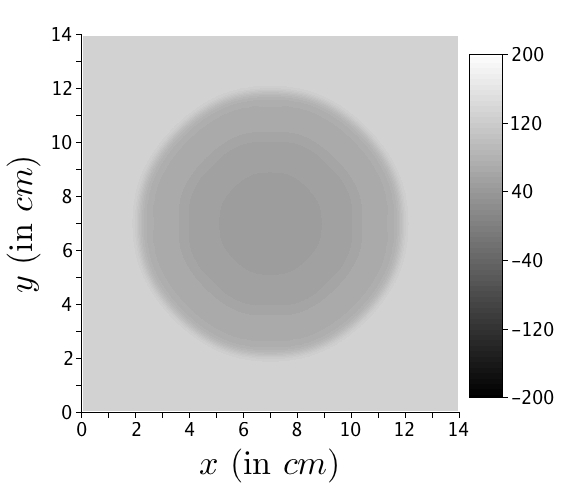
\includegraphics[width=0.45\textwidth]{simu/trefle_track/track_14x14_cross/vue_scan/vue_scan84.png}}
\subfloat[Evolution (in days) of tumor area (in $mm^2$).]{
\label{fig:evo_aire_cross}
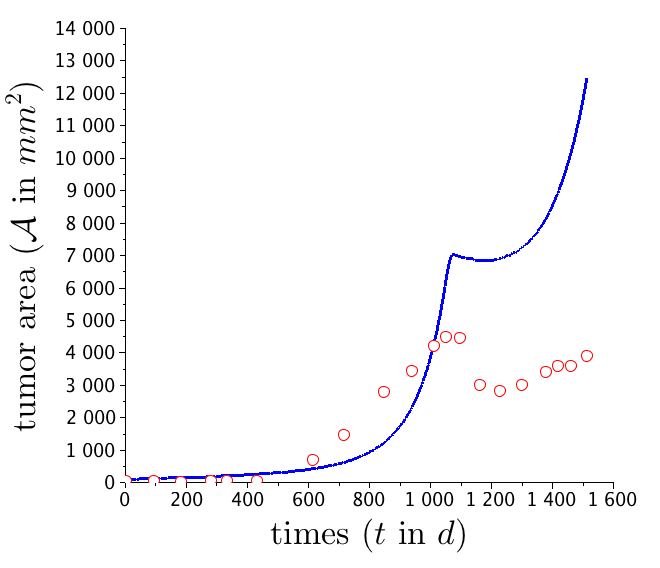
\includegraphics[width=0.45\textwidth]{simu/trefle_track/track_14x14_cross/fit_area.png}}
\caption{\label{fig:correction_cross}Numerical simulation with
    \twinweno\  scheme ($\beta=0.26$) with the same parameters as for Figure~\ref{fig:simu_chen_cross0_scan} . The numerical tumor area does
    not fit with the data.}
\end{figure}
%
%%%%%%%%% Modification des param avec twin weno 5

\begin{figure}
%\vspace{-6mm}
\subfloat[Day 0]{
\includegraphics[width=0.32\textwidth]{simu/fit_chen7_L12_cross0.3/vue_scan/vue_scan1.png}}
\subfloat[Day 424]{
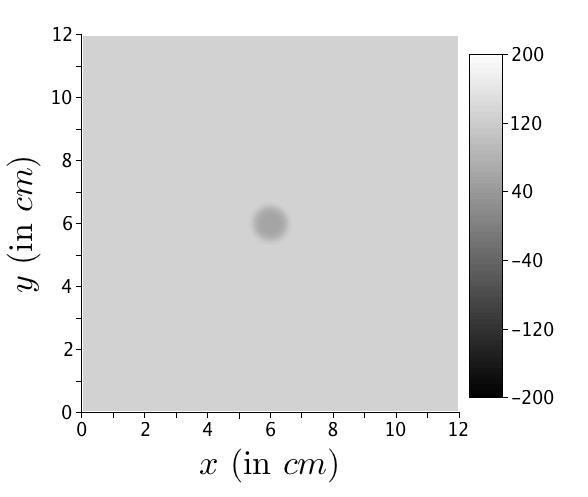
\includegraphics[width=0.32\textwidth]{simu/fit_chen7_L12_cross0.3/vue_scan/vue_scan26.png}}
\subfloat[Day 849]{
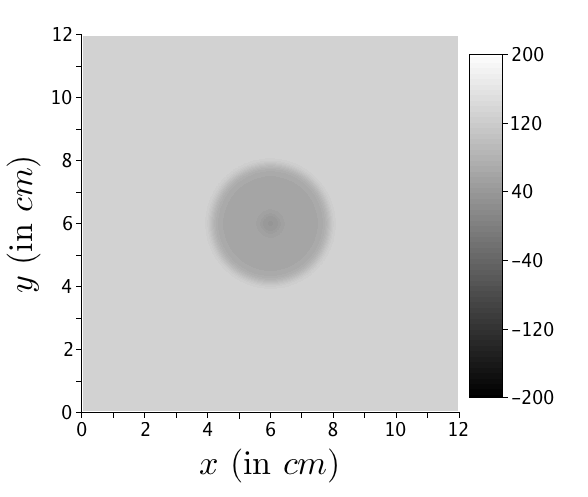
\includegraphics[width=0.32\textwidth]{simu/fit_chen7_L12_cross0.3/vue_scan/vue_scan51.png}}\\
%\vspace{-4mm}
\subfloat[Day 1052]{
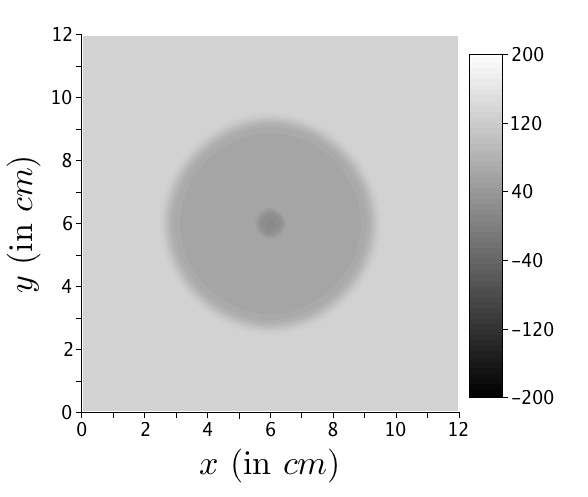
\includegraphics[width=0.32\textwidth]{simu/fit_chen7_L12_cross0.3/vue_scan/vue_scan63.png}}
\subfloat[Day 1222]{
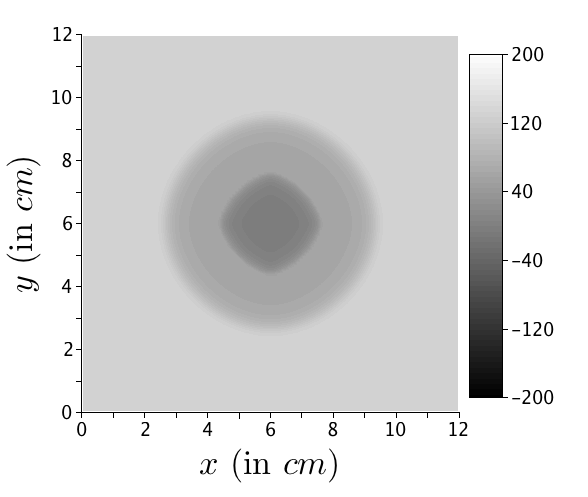
\includegraphics[width=0.32\textwidth]{simu/fit_chen7_L12_cross0.3/vue_scan/vue_scan73.png}}
\subfloat[Day 1460]{
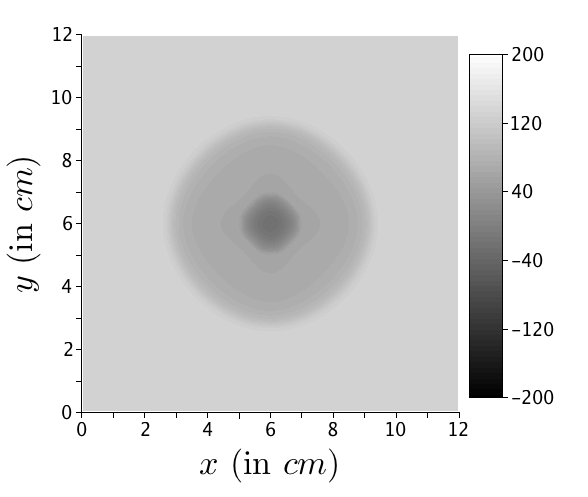
\includegraphics[width=0.32\textwidth]{simu/fit_chen7_L12_cross0.3/vue_scan/vue_scan87.png}}
\caption{Numerical simulations with \twinweno\ ($\beta=0.3$)
    for patient B with fitted parameters on the tumor area: spatial evolution of the lesion with numerical reconstitution of CT-scans.\\
The unit of grey scale is arbitrary. \label{fig:simu_chen_cross0.3_scan}}
\end{figure}


%%%%%%% Figure variation dose traitement

\begin{figure}[!htb]
%%\vspace{-6mm}
\subfloat[Progression free survival time ($T_{PFS}$ in days) as a function of  $\delta$.]{
\label{fig:Tmaintien_chen}
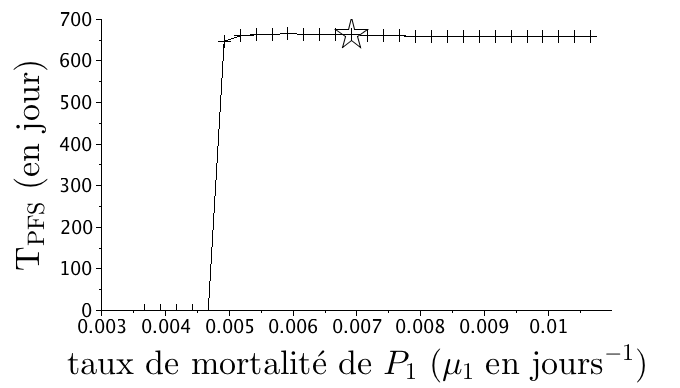
\includegraphics[width=0.5\textwidth]{DB-chen-eff-glivec/Tmaintien.png}}
\subfloat[Time corresponding to the growth of tumor area by a factor 2
($T_{double}$ in days) as a function of $\delta$.]{
\label{fig:Tdouble_chen}
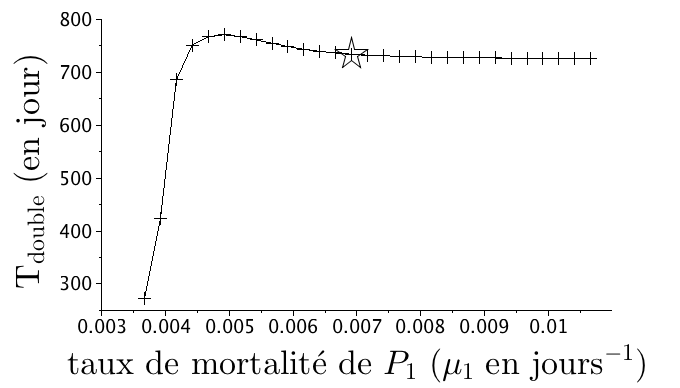
\includegraphics[width=0.5\textwidth]{DB-chen-eff-glivec/Tdouble.png}}\\
\subfloat[Minimal area reached ($\mathcal{A}_{min}$ in $mm^2$) as a function of  $\delta$.]{
\label{fig:Amin_chen}
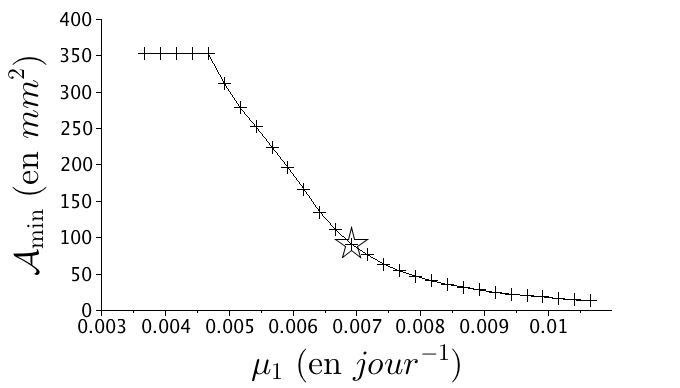
\includegraphics[width=0.5\textwidth]{DB-chen-eff-glivec/Amin.png}}
\subfloat[Phase portrait.]{
\label{fig:portrait_phase_chen}
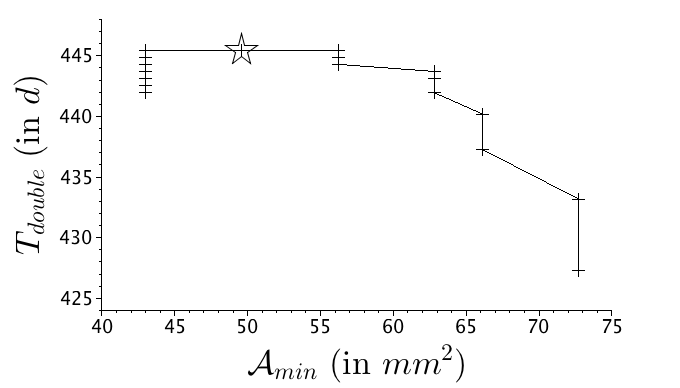
\includegraphics[width=0.5\textwidth]{DB-chen-eff-glivec/portrait_phase.png}}
\caption{matinib efficiency on patient B.\\
The star corresponds to the parameters used in Figure~\ref{fig:fit_area_chen} for the fit of the tumor area. \label{fig:eff_glivec_chen}}
\end{figure}

\end{document}